% -*- coding: UTF-8 -*-
% hello.tex

\documentclass[UTF8]{book}

\usepackage{xeCJK}
\usepackage[utf8]{inputenc}

\usepackage{hyperref}
\hypersetup{pdftex,colorlinks=true,allcolors=blue}
\usepackage{hypcap}

\usepackage{color}
\usepackage[usenames, dvipsnames, svgnames, table]{xcolor}
% \pagecolor{gray}

\usepackage{makeidx}
\makeindex

\usepackage{amsmath}
\usepackage{mathtools}

\usepackage{listings}
\usepackage{multicol}
\usepackage{fancybox}
\usepackage{tcolorbox}
\usepackage{enumitem}

\usepackage{indentfirst}

% table
\setlength{\arrayrulewidth}{1pt}
\setlength{\tabcolsep}{16pt}
\renewcommand{\arraystretch}{2.5}
\newcolumntype{s}{>{\columncolor[HTML]{AAACED}} p{3cm}}

\arrayrulecolor[HTML]{DB5800}

\title{LICH架构文档}
\author{董冠军}
\date{\today}

% \bibliographystyle{plain}
% \bibliography{math}

\begin{document}

\maketitle
\tableofcontents

\part{任务清单}

\chapter{任务清单}

%\pagestyle{empty}
\todo[inline]{The original todo note withouth changed colours.\newline Here's another line.}
\lipsum[11]\unsure{Is this correct?}\unsure{I'm unsure about also!}
\lipsum[11]\change{Change this!}
\lipsum[11]\info{This can help me in chapter seven!}
\lipsum[11]\improvement{This really needs to be improved!\newline\newline What was I thinking?!}
\lipsum[11]
\thiswillnotshow{This is hidden since option `disable' is chosen!}
\improvement[inline]{The following section needs to be rewritten!}
\lipsum[11]
%\newpage

\section{原生卷}

\begin{tcolorbox}
\begin{compactenum}
    \item 存储池
    \item 数据恢复性能
    \item \sout{async sqlite}
    \item \hlc{batch sqlite}
    \item Allocate的性能
    \item 精简配置,快照对性能的影响
    \item 快照树
    \item 单卷快照的数量
    \item SSD Cache
    \item Redis Cache
    \item 异步远程复制
    \item VAAI
    \item FC (+VAAI)
\end{compactenum}
\end{tcolorbox}

\section{关键特性和过程}

\begin{compactenum}
    \item flush, load and recovery
    \item 保护模式 safe mode
    \item 存储分层
    \item 命令行工具,扩展卷和快照相关操作到LSV
\end{compactenum}

\section{兼容性}

\begin{compactenum}
    \item 版本演进
\end{compactenum}

\section{Pool}

\begin{compactenum}
    \item Resource Pool
\end{compactenum}

\section{Volume}

\begin{compactenum}
    \item new format: row2
    \item new format: lsv
    \item vol max size 256T+
    \item vol resize?
    \item all zero's chunk
\end{compactenum}

\section{快照}

\begin{compactenum}
    \item 支持60000+快照
    \item consistency group
    \item 每个snap的大小等信息
    \item snap大小对GC策略的影响
\end{compactenum}

\section{一致性/正确性}

\begin{tcolorbox}
\begin{compactenum}
    \item 底层数据检验工具(chunk0, volume, log/gc, bitmap, wal, rcache)
    \item 内置质量,各模块添加自校验机制,方便诊断数据正确性问题(assert + log + test)
    \item 加强断言:pre和post条件,变量变化规则,不变式,基本假设等
    \item 日志用tag/keywork和timeline,以便于跟踪一个对象的变化历史,用一个或多个维度贯穿起来,用于辅助诊断
    \item 增加CHUNK\_HISTORY,以时间线方式,跟踪记录CHUNK变化的生命周期
\end{compactenum}
\end{tcolorbox}

\section{性能}

性能是负载和资源的函数, $P=F(W, R)$。

\begin{tcolorbox}
\begin{compactenum}
    \item 创建卷时,rcache分配了4096M的SSD cache,可以延迟分配
    \item \textcolor{red}{rcache 顺序IO随机化问题}
    \item wbuf 顺序IO随机化问题
    \item 系统启动时间
    \item 预填充lich chunk
    \item GC策略和算法
    \item 统计基础操作的开销,作为性能分析的基础
\end{compactenum}
\end{tcolorbox}

\section{负载}

\begin{tcolorbox}
\begin{compactenum}
    \item IO队列深度
    \item IO平均大小
    \item IO读写大小
\end{compactenum}
\end{tcolorbox}

\section{资源}

\begin{tcolorbox}
\begin{compactitem}
    \item 内存使用量过大
    \item 内存泄漏
    \item 磁盘利用率不足
    \item 网络带宽:瓶颈或利用率不足
    \item 中断
    \item soft lock up?
\end{compactitem}
\end{tcolorbox}

\section{故障处理}

\begin{compactenum}
    \item \change{故障域,不能中断IO}
    \item 节点间负载均衡(<20\%)
\end{compactenum}

\section{Misc}

\begin{tcolorbox}
\begin{compactitem}
    \item FC
    \item Remote copy
    \item SSD cache
    \item EC
    \item 有效容量的比例
    \item 热插拔
    \item 磁盘漫游
    \item 在线扩容
    \item 滚动升级
\end{compactitem}
\end{tcolorbox}

\section{DONE}

\begin{compactenum}
    \item VAAI [+xcopy]
\end{compactenum}


\part{FusionStorage}

\chapter{模型}

\begin{tikzpicture}[show background grid]
    \begin{class}{Disk}{6, 0}
    \end{class}
    \begin{class}{Pool}{6, 2}
    \end{class}
    \begin{class}{Volume}{6, 4}
    \end{class}
    \begin{class}{Host}{6, 6}
    \end{class}
    \begin{class}{Cluster}{0, 2}
    \end{class}
    \begin{class}{Snapshot}{0, 4}
    \end{class}

    \composition{Cluster}{pools}{1..*}{Pool}
    \composition{Pool}{disks}{1..*}{Disk}
    \composition{Pool}{volumes}{1..*}{Volume}
    \composition{Volume}{mapping}{*..*}{Host}
    \composition{Volume}{snapshots}{1..*}{Snapshot}
\end{tikzpicture}

\section{Cluster}

整体

\section{Pool}

把物理节点划分为不同的保护域,一个卷的所有数据只出现在一个保护域内。卷可以跨保护域进行复制和迁移。

默认一个,包括所有节点。

% 保护域是物理节点的划分,存储池是存储介质的划分。每块盘只能出现在一个存储池里。

Pool: 逻辑容器

故障域有粒度之分,如磁盘,节点,机架,机柜,数据中心。

存储池内,要满足故障域规则:一个chunk的不同副本,分布在不同的故障域内。\label{rule:faultset}

在初次分配,再平衡和恢复等过程中,都需遵循这些规则。

\begin{tcolorbox}

可以参考ceph的CRUSH实现。bucket和device定义了集群的物理拓扑结构,rule定义了数据存取规则,
pool上关联rule,从而定义了pool中卷数据的放置规则。设备即OSD,对应一个物理磁盘。

***

存储池可以取代保护域,定义所有对象的存放位置是一个节点集。

***

存储池可以用来实现tier cache。重定向IO到cache pool。

***

统一概念:保护域,故障域,存储池,pool。Consistency Group不同于pool,与物理存取无关,
而是卷的逻辑集合,卷可以来自不同的pool。

\end{tcolorbox}

与存储池有什么同和异?存储池可以看做关联了磁盘的pool,可以看做pool的子类。

属性:
\begin{enumbox}
\item 配额
\item 复制类型:副本 OR EC
\item 磁盘列表
\item 定义精简池
\item 存储池上可以指定卷的副本数
\item \hl{有足够的故障域,且不同故障域配置一致的资源量}
\end{enumbox}

操作:
\begin{enumbox}
\item 创建
\item 删除
\item 扩展(添加磁盘到\hl{已存在的存储池},该映射关系持久化到本地,同步到admin节点)
\item 缩容(从存储池中移除磁盘,引发数据重建过程)
\item \hl{自动或手动按磁盘速率进行存储池分级划分}
\item 不同存储池之间,卷的复制
\item 不同存储池之间,卷的迁移,可在线或离线
\item 存储池级别的统计信息
\end{enumbox}

% 存储池是disk的集合,与节点无关。但disk所在的节点构成存储池的节点列表,不同存储池的节点可能覆盖。

存储池下,可以创建volume。没有关联磁盘的存储池,不能创建卷。

\hl{chunkid到磁盘物理位置有两级映射:chunk的副本节点列表,节点内chunkid到物理地址的映射}。

在为卷分配chunk的时候,需要确定各个副本的物理存储位置。当前实现是返回不同副本的节点列表。
如果指定了存储池,就需要在存储池所在的节点范围内进行分配。同时要满足故障域和数据均衡规则。

\begin{tcolorbox}
移动采集中存储池要求,相比于目前的逻辑pool,更多是一种设计上的退步。
存储虚拟化的目标,是物理位置无关。我们可以基于逻辑容器,实现基于策略的管理。
所以,\hl{从实现层面,要保留当前pool的功能,按照系统配置确定pool的类型}。
\end{tcolorbox}

% 存储池内,要满足故障域规则(\ref{rule:faultset})

步骤:
\begin{enumbox}
\item 创建pool,但此时不能创建pool的元数据chunk,因为还没有绑定磁盘(需要一全局的地方,存储pool名字)
\item 添加磁盘到pool,通知admin节点
\item 当在pool下面创建卷的时候,前提条件是已准备好磁盘,生成pool元数据chunk(位于同一pool里)。
\end{enumbox}

pool元数据chunk必须位于自己的存储池内,如果分布在不同的存储池,不满足故障域条件。

pool引导信息可以存在rootable里。

\section{Volume}

属性:

操作:
\begin{compactenum}
    \item rename
    \item resize \info{在线扩容}
    \item mv
    \item copy \change{全量拷贝/增量拷贝} \change{跨存储池拷贝} % change不能出现在box里
\end{compactenum}

\section{Snapshot}

snapshot隶属于卷,无卷则无快照,快照组织成快照树,其中有且只有一个快照是可写快照,即卷的写入点。

\section{Mapping}

数据隔离/ACL,数据保护

卷对主机的可见性。一个卷只有映射给了某主机,才可以被该主机访问。


\section{Consistency Group}

一致性卷组

\begin{shadequote}
Consistency Groups could be useful for Data Protection (snapshots, backups) and
Remote Replication (Mirroring).

The Mirroring support will allow to setup mirroring of multiple volumes in the
same consistency group (i.e. attaching multiple RBD images to the same journal
to ensure consistent replay).

There is already an interest to implement this functionality as a part Mirroring feature:
http://tracker.ceph.com/issues/13295

The snapshot support will allow snapshots of multiple volumes in the same
consistency group to be taken at the same point-in-time to ensure data
consistency.
\end{shadequote}

\chapter{硬件架构}

\section{节点}

\subsection{添加节点}

负载均衡,需要重新平衡数据

\subsection{删除节点}

恢复


\section{Pool}

\section{Disk}

\subsection{Tool}

操作磁盘的工具
\begin{enumbox}
\item hdparm set/get hard disk parameters
\item iostat
\item lsscsi
\item udevadm
\item sg\_inq
\item disk2lid
\end{enumbox}

\subsection{Cache}

Disk Cache

关闭磁盘cache,防止出现数据不一致情况。怎么关闭呢?相关管理工具是什么?

磁盘的设备驱动,linux kernel的块设备IO架构

NVMe具有什么特征?

\subsection{RAID}

Ctrl+R进入bios的RAID控制界面。通过bios进行的管理操作,进入系统后用MegaCli等命令行工具也能完成。
且更为方便。

每个控制器管理一个或多个enclosure,每个enclosure有固定数量的slot。每个slot对应一块物理设备。
每个物理设备处在不同的firm 状态,这些状态可以相互转换。在物理设备之上,构建虚拟设备。

带电池BBU的情况下,可以打开RAID cache。

NVMe在不在RAID里,系统盘呢?看不到系统盘,是因为系统盘不在RAID控制器管理的slot内?

缓存盘做出JBOD,数据盘RAID0

全部是JBOD,性能影响较大。

\subsection{Tier}

检测磁盘分层,支持两个磁盘分层:0和1, 0是SSD,1是HDD。

\subsection{Meta}

磁盘管理元数据目录:/opt/fusionstack/data/disk:
\begin{compactitem}
\item disk
\item \hl{bitmap}
\item info
\item tier
\end{compactitem}

对每块磁盘,开头的1M是引导信息,通过bitmap来进行空间管理。
引导信息包含了所在节点信息,所以只能在节点内进行磁盘漫游。

所在源文件是\emph{diskmd.c}。调用fnotify\_register监控磁盘目录的变化,进而添加或移除相应磁盘。

每个节点最多可以添加256个磁盘。

sqlite3划分为10个db文件,chkid信息hash到相应的db。每个db包含两个table:metadata和raw。

\begin{lstlisting}[frame=single]
CREATE TABLE metadata (key text primary key, 
    disk integer, 
    offset integer, 
    parent text, 
    priority integer, 
    meta_version integer, 
    fingerprint integer, 
    wbdisk integer);

CREATE TABLE raw (key text primary key, 
    disk integer, 
    offset integer, 
    parent text, 
    priority integer, 
    meta_version integer, 
    fingerprint integer, 
    wbdisk integer);
\end{lstlisting}

\subsection{状态机}

拔盘-恢复未完成,如何加入?(符号链接丢失,别的文件处在可用状态,重启lichd,修复符号链接)

拔盘-恢复完成,如何加入?

\section{Advanced}

NVMe

RDMA/DPDK/SPDK

AFA

\chapter{优化项}

\section{时间优化}

\begin{itemize}
    \item localize
    \item auto tier
    \item ssd cache
\end{itemize}

\section{空间优化}

\begin{itemize}
    \item 精简配置 (Thin provisioning)
    \item EC
    \item Dedup
    \item Compress
\end{itemize}



\chapter{快照和克隆}

\chapter{企业级特性}

\section{Security}

iscsi CHAP认证

\section{QOS}

token bucket

\change{距离函数}


\section{Quota}

\section{Multipath}

\section{DR}

snapshot

io journalling

\section{CDP}

\chapter{LSV}

现有Lich raw卷,存在性能问题,COW快照也不便于扩展。所以实现了Log structured Volume,
转化随机IO为顺序IO,基于其上,实现了ROW快照。

特别要注意的是,实现中应着力避免顺序IO随机化,会引起IO放大,从而极大地降低性能。


\section{Volume}

Volume模块负责空间管理。提供malloc/free接口,也可批量分配和回收。采用bitmap和free list多种管理方式。
freelist充当分配缓冲区的角色,可持久化,也可不持久化。

lsv-lich raw-disk的chunk空间存在两级映射关系,会影响到读写性能。

底层空间宜按固定大小的段来组织。每个段空间管理的开销是固定的。
目前支持两级存储分级:
\begin{tcolorbox}
    \begin{multicols}{2}
        \begin{itemize}
            \item 0:ssd
            \item 1:hdd
        \end{itemize}
    \end{multicols}
\end{tcolorbox}

\section{Bitmap}

Bitmap更合适的叫法是页表,与操作系统里的页表类似,负责虚拟地址到物理地址的映射关系。Bitmap有两层:L1和L2,
按类似页表的方式组织。和Log层数据一起,构成三层。

L1是Bitmap的头部,大小固定,属于卷或快照私有。L2按需分配,在快照之间共享。在Clone的情况下,会涉及跨卷读。

通过Bitmap层,支持快照的全部特性,多个快照构成快照树。快照树分两种方式展示:树状或列表。

\section{Log/Chunk}

底层物理空间,划分为固定大小为1M的数据块,进行统一管理:分配/释放。

在Volume模块之上做了简单封装,表示卷的数据,Bitmap表示卷的元数据。在覆盖更新的情况下,Bitmap指向新的数据页,
导致原来的数据页失效,可以回收。在有快照的情况下,会变得较为复杂。

Log模块无需要持久化的信息。

在Lich卷空间映射到磁盘的时候,目前实现为一个随机过程。\textcolor{red}{磁盘的1M随机和顺序,差别较大}。

\section{WBuf}

Wbuf有两个序列:WAL和Wbuf的提交序。在wbuf中读出的最新数据和提交后通过bitmap+log读取的数据,应该一致。

IO内,LBA不同,无冲突,页序;IO间,LBA可能相同,有冲突,需要串行化。

\section{RCache}

多级缓存机制,需要注意针对多种读场景进行优化,如顺序读。因为经过虚拟页表映射,虚拟地址空间和物理地址空间,顺序可能是交叉的。
应着力避免出现顺序变随机导致读放大的情况。

预读很重要,也比较困难,需要构建学习模型。

\section{GC}

log功能单一化,gc模块独立出来。gc要解决的问题有二:
\begin{enumerate}
    \item 跟踪所有log
    \item 在所有log中,根据一定策略(qos),选择回收价值最大者进行回收
\end{enumerate}

目前的实现,是局域的解,而不是全局最优解,是bottom-up的分代垃圾回收器。可增量并行执行,与前台赋值器需要同步机制。
回收器和赋值器需要读写barrier。

优化GC Check过程:每一页的信息,只会出现在部分的bitmap记录里,与快照树的拓扑结构有关。
在创建快照时,分配snap id。 snap id组织成单调递增的序列。如果中间没有删除或rollback操作,
很容易定位到某页所属的快照点。经过rm或rollback之后,情况有所不同,但依然有迹可循。

\section{Recovery}

正常关机的情况下,各个模块会flush必要的数据,下次启动的时候,load出来即可。

异常关机的情况下,各个模块没有机会flush数据,导致丢失部分内存状态信息。
这样,在下次启动的时候,需要执行恢复过程。

需要flush数据的模块有:
\begin{itemize}
    \item Wbuf
    \item GC
    \item Volume
\end{itemize}

提出几个问题:
\begin{tcolorbox}
\begin{enumerate}
    \item 正常关机时,需要flush什么信息?
    \item 恢复过程,从X恢复出Y,X是什么?Y是什么?(X是日志,Y是最新状态)
    \item 怎么理解提交等基础操作?
    \item 恢复的性能如何?如何通过检查点机制改善恢复性能?
\end{enumerate}
\end{tcolorbox}

针对以上问题,每个模块的恢复机制有所不同,但分析方法具有通用性。

\subsubsection{Volume Recovery}

 $U = (A - B) + C + D$

tail标记了可见空间,可见空间=已分配+可分配(free list)。free list组织成内存和磁盘两部分。flush时,需要持久化freelist的内存部分。

在调用malloc和free接口的时候,会同步更新用于空间管理的bitmap。为1的为已分配,为0的为可分配,这个关系总成立。

为了支持批量malloc和free接口,引入dirty page bitmap,类似于GC中提到的卡表,可以实现\textcolor{red}{多次更新,一次提交}的设计模式。

主要操作:
\begin{tcolorbox}
\begin{itemize}
    \item malloc操作:依次从C,D,U里取可用chunk。
    \item free操作:把释放的chunk放入C,如果C满,则转化为D。
\end{itemize}
\end{tcolorbox}

这里的提交操作可以理解为:C转化为D的过程,并没有记录检查点。
所以恢复操作,要全扫描bitmap,从bitmap重建C和D。

\subsubsection{GC Recovery}

GC recovery过程可以理解为:从gc bitmap重建内存状态。

所有的log,分为两部分:old storage和bitmap。bitmap相当于journalling。进入check queue的logctrl,先登记到bitmap。
在提交时,即从heap移入old storage时,清除/注销相应的bitmap项。

\subsubsection{Wbuf Recovery}

谁充当了日志的角色?在wbuf模块很明确,有专门的WAL。写入阶段登记,commit阶段回收。

\section{LSV测试}

LSV(\textcolor{red}{Log Structured Volume})基于Lich原生卷,实现了日志结构的卷格式,支持快照的各种操作。

相对于Lich原生卷,LSV有几点优势:
\begin{tcolorbox}
    \begin{itemize}
        \item 转化随机IO为顺序IO,混合存储情况下有更高性能
        \item 实现为ROW快照,zero-copy快照,\textcolor{red}{支持快照树}
    \end{itemize}
\end{tcolorbox}

LSV的关键过程:
\begin{tcolorbox}
    \begin{description}[style=nextline]
        \item [写] 写入wal和wbuf后,即可返回。wbuf积聚到1M时,提交log+bitmap后台异步任务。
        \item [读] 从wbuf读取最新数据,如果没有命中,则依次从rcache,bitmap+log读取。
        \item [GC] 垃圾回收,后台异步任务,按一定策略,回收无效页。
        \item [重启] 分两种情况,正常和异常情况。正常情况下会刷新内存状态,重启时直接加载即可;异常情况下,进入recovery过程。
    \end{description}
\end{tcolorbox}


LSV测试,主要分为功能,正确性和性能几个方面,\textcolor{red}{正确性和性能按标准测试用例}执行即可。下面列出一期测试计划。

\subsubsection{GIT分支}

lsv\_pipeline

\subsubsection{特性}

%\begin{tcolorbox}
\begin{lstlisting}[language=bash,frame=single]
# 创建LSV卷:
lichbd vol create p1/v1 --size 100Gi -F lsv -p iscsi

# 快照功能,与原来一样,部分命令示例:
lichbd snap create p1/v1@snap1 -p iscsi
lichbd snap create p1/v1@snap2 -p iscsi
lichbd snap ls p1/v1 -p iscsi

# 暂不支持flat操作

\end{lstlisting}
%\end{tcolorbox}

\subsubsection{性能/正确性测试清单}

\begin{itemize}
    \item 与lich原生卷全面的性能对比
    \item 资源利用率(包括磁盘,内存)
    \item 系统启动时间
    \item 重启系统的恢复过程
    \item 存储分层
    \item 扩展到多卷
\end{itemize}

\subsubsection{注意事项}

\begin{itemize}
    \item 日志满:/opt/fusionstack/log/lich.log (echo 5 > /dev/shm/lich4/msgctl/level)
\end{itemize}


\chapter{实现}

\section{Schedule}

不能支持嵌套task,用pre yield变量来控制。

\section{内存}

提供什么接口,三种生命周期范围、持久性:
\begin{easylist}[itemize]
& 常驻
& session
& IO
\end{easylist}


使用场景
\begin{easylist}[itemize]
    & core private memory
    & sche\_task
    & RDMA
    & buffer\_t
    && libnvme
    & little object
    & ring
\end{easylist}

采用buddy算法管理连续内存分配

动态化

用面向对象的方式处理,每个core对应一个MR对象。public的也是如此。

每个对象内嵌一个buddy对象管理hugepage的分配、释放。
另外,从core的MR里,利用buddy算法分配连续内存,用于ring等小对象。

禁止在一个core内malloc,由另外一个core进行free。

怎么抽象一般内存和hugepage-based内存?

抽象出head,core和public重用代码。第一选择head,第二执行head的操作。

\subsection{buffer}

\begin{center}
    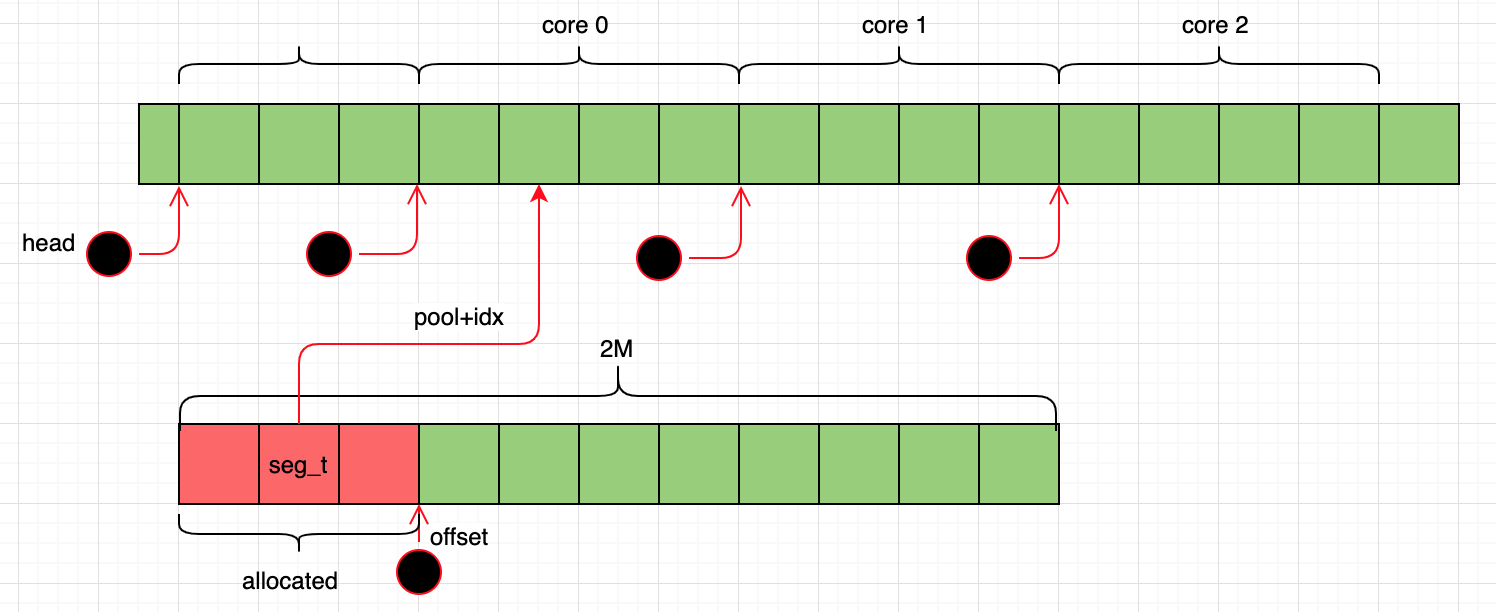
\includegraphics[width=10cm]{../imgs/buffer-t.png}
\end{center}

每个内存区域的\hl{第一个hugepage用来保存该区域的元数据信息},可供分配的是后面的hugepages。
在元数据信息中加上buddy,可用来支持buddy算法。

buffer的每个seg都包含有虚拟地址和物理地址。

\subsection{Memory Pool}

\begin{center}
    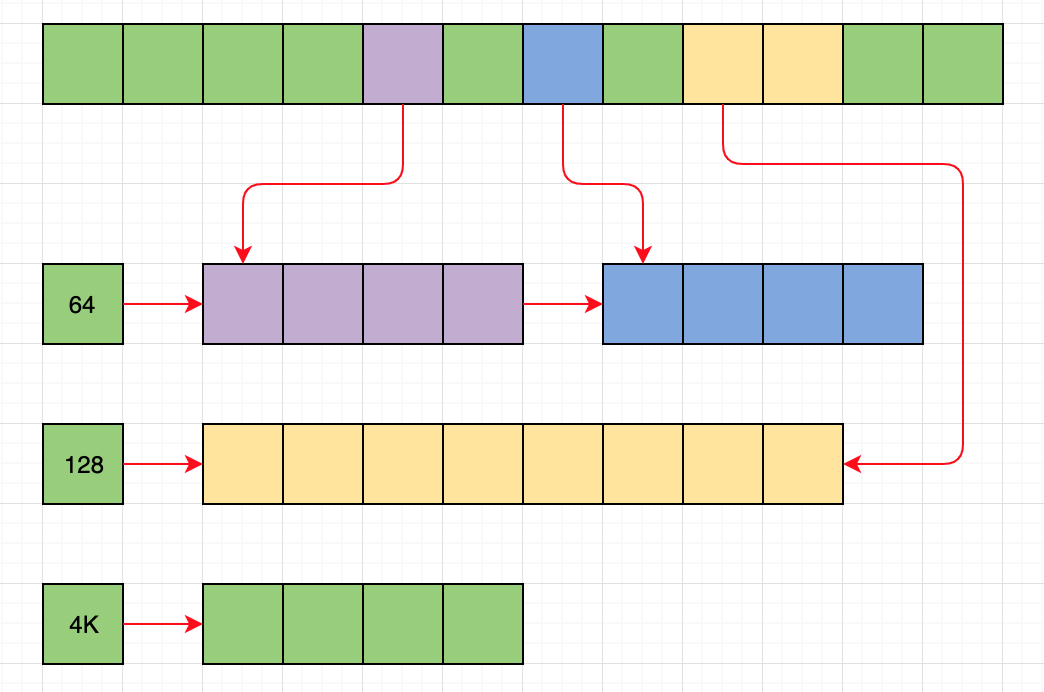
\includegraphics[width=10cm]{../imgs/memory-pool.png}
\end{center}

直接从hugepage申请内存,从hugepage申请一个hugepage,用于小对象。pool管理多个size的小对象队列。
根据要malloc的size,定位到队列。

free时按指针查找属于哪个hugepage。每个hugepge对应起始地址和结束地址以及所在队列的标识。
这样可以保留malloc和free的语法和语义。

hugepage层只需要提供分配单个hugepage的接口,一个队列可以由一个或多个hugepage构成。

或者,memory pool按4k进行组织,同样采用buddy算法。在其上实现ring等。

\hl{每layer都要动态化,包括增和减}。

\subsection{NVMe}

NVMe为什么需要物理地址?

direct io需要512对齐。

\subsection{RDMA}

每个连接$1024*512$内存。

\subsection{IO}

\begin{center}
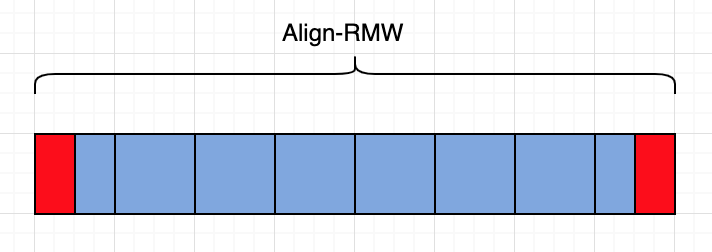
\includegraphics[width=10cm]{../imgs/io-align.png}
\end{center}

首尾页对齐

buffer\_t包含一个seg时,方便处理。如果有多个seg,是否需要分配连续的大块内存。

\hl{SPDK的大IO问题}:NVMe需要物理内存,并且一次io物理内存是连续的。
malloc的内存,不容易找到物理内存。
2M的hugepage虽然能获取虚拟地址连续的4M地址空间,但底层物理内存未必连续。
用1G的hugepage更容易管理。

GFM的机制是什么?barrier去解决RMW、chunk恢复等问题?

\chapter{FAQ}

问题集:
\begin{enumbox}
\item /的位置信息
\item 当前分配的最大卷ID?
\end{enumbox}

P1: IOMeter测试,256K,Lich顺序和随机IO性能差别大

P2: lsv\_gc\_check断言失败

P3: Error Handling


\part{基础理论}

\chapter{分布式系统}

Lich涉及许多底层理论和系统,包括并行计算和分布式系统,操作系统,文件系统,数据库系统,网络,还包括相应的底层硬件架构。
需要对数据结构和算法,有良好基础。所以,对基本问题和理论,要有清晰和深入的掌握,才能“运用之妙,存乎一心”。

存储中一些重要的问题,可以借助AI的力量去解决。智能存储,不仅仅是口号,更是技术进步的必要趋势。

按道法术器组织结构,写成大文章。

常用优化原则:
\begin{itemize}
    \item 局部性
    \item 并行
    \item 聚合,批处理
    \item 延迟
\end{itemize}

\chapter{Parallel Computing}

pattern
\begin{itemize}
    \item pipeline
    \item fork and join
\end{itemize}

\chapter{Design Pattern}

\begin{itemize}
    \item journalling
    \item update many, commit one
    \item double check
    \item double/multi buffer
    \item half sync, half async
\end{itemize}


\end{document}
